%%%%%%%%%%%%%%%%%%%%%%%%%%%%%%%%%%%%%%%%%%%%%%%%%%%%%%%%%%%%%%%%%
% Dissertacao de Mestrado / Dept Fisica, CFM, UFSC              %
% Lacerda@UFSC - 2013                                           %
%%%%%%%%%%%%%%%%%%%%%%%%%%%%%%%%%%%%%%%%%%%%%%%%%%%%%%%%%%%%%%%%%

%:::::::::::::::::::::::::::::::::::::::::::::::::::::::::::::::%
%                                                               %
%                          Capítulo 3                           %
%                                                               %
%:::::::::::::::::::::::::::::::::::::::::::::::::::::::::::::::%

%***************************************************************%
%                                                               %
%                      PCA e Tomografia PCA                     %
%                                                               %
%***************************************************************%

\chapter{PCA e Tomografia PCA}
\label{sec:PCAeTomoPCA}

De medidas fisiológicas, como pulsação e respiração, até reconhecimento de padrões em sistemas complexos como
reconhecimento facial e criptografia, passando por compactação de imagem, neurosciência e redução de ruídos em dados,
podemos ver atuação de técnicas de PCA. Neste capítulo revisamos os fundamentos matemáticos da PCA e de sua versão para
cubos de dados (Tomografia PCA).

%***************************************************************% 
%                                                               %
%                              PCA                              %
%                                                               % 
%***************************************************************%

\section{Análise de Componentes Principais}
\label{sec:PCAeTomoPCA:PCA}

Baseada em encontrar o eixo com maior variância em um conjunto de variáveis (no nosso caso, fluxos por lambda e por zona
espacial) e gerar, a partir dele, uma base ortogonal e normalizada, a técnica de PCA vem sendo de grande utilidade
quando o assunto é estatística com muitas variáveis. Através de operações relativamente simples, utilizando álgebra
linear podemos obter essa nova base. Com a nova base podemos realizar a projeção dos dados observados nela, como uma
rotação na base de dados original, gerando um novo conjunto de dados não correlacionados linearmente.

Existem diversas formas de se calcular essa base final. A prova matemática que você pode obter essa base é feita através
de multiplicadores de Lagrange, calculando os autovetores ($\mathbf{e}{}_k$) e autovalores ($\Lambda_k$) que maximizam o
valor de $\mathbf{e}{}_k^T \cdot \mathbf{C}{}_{cov} \cdot \mathbf{e}{}_k$ (ver Eq. \ref{eq:PCA:covMatrix}) sujeito à
restrição de que um autovetor deve ser ortogonal a qualquer outro da base ($\mathbf{e}{}_i^T \mathbf{e}{}_j = 0$) e que
todos devem ser normalizados ($\mathbf{e}{}_i{}^T \mathbf{e}{}_i = 1$) \citep[][p. 5-6]{JolliffePCA1986}. No caso de PCA
com espectros, o fluxo em cada comprimento de onda varia através das zonas. Encontramos então quais são os eixos mais
significativos desse espaço em relação à variância, sujeitos às restrições acima. Fazemos esse cálculo encontrando os
autovetores e autovalores da matriz de covariância (a matriz tem dimensão $N_\lambda \times N_\lambda$) usando a
biblioteca científica \texttt{SciPy}\footnote{\url{http://scipy.org/}}.

Para exemplificar em uma forma visualizável (Figura \ref{fig:PCA:exempl2D}), imaginemos que todos os espectros que temos
possuem apenas dois comprimentos de onda ($N_\lambda\ =\ 2$). Podemos então gerar um gráfico num plano cartesiano
($\lambda_1 \times \lambda_2$) onde cada ponto representa um espectro. A primeira componente principal (PC) está na
direção que possui maior variância nos dados, e a segunda, é a que possui maior variância, com a limitação de ser
ortonormal a primeira PC.

\begin{figure}
    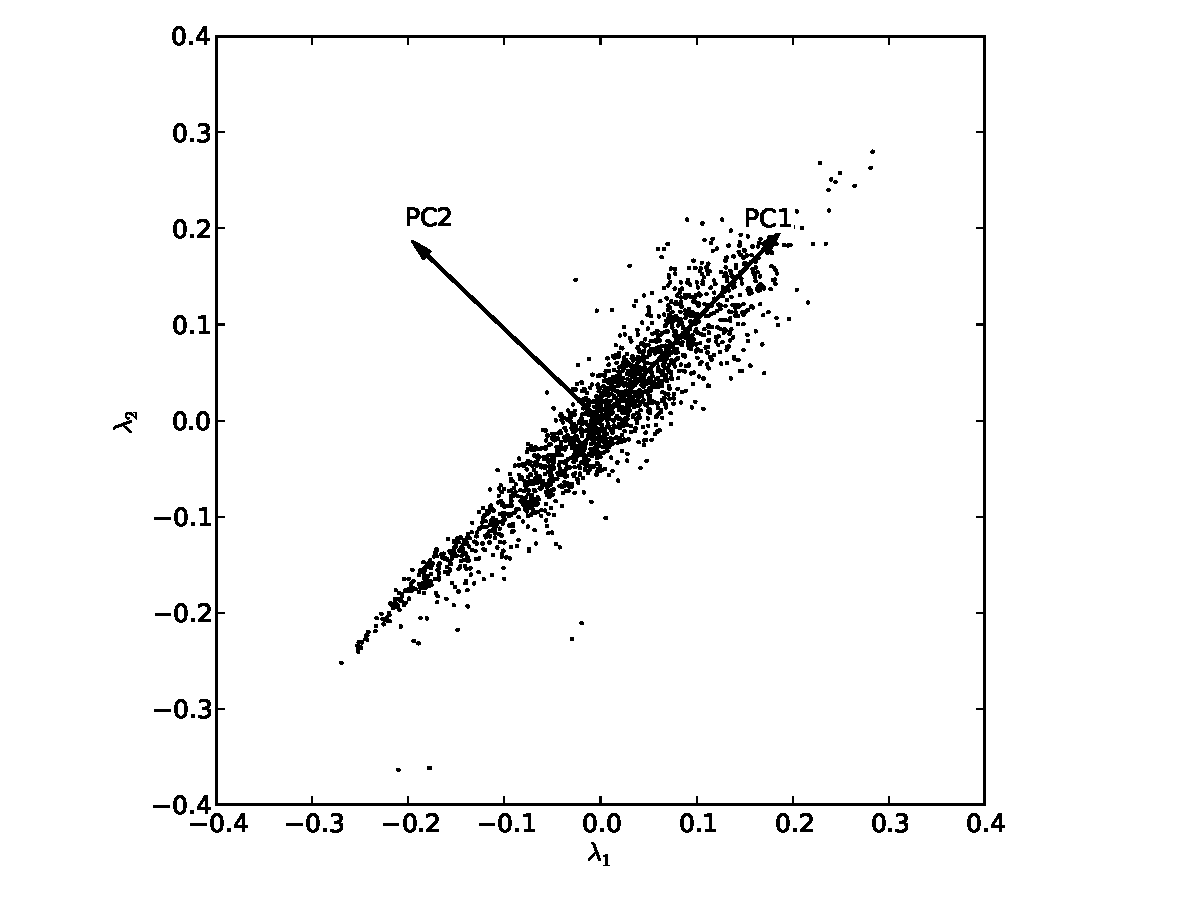
\includegraphics[width=0.8\textwidth]{figuras/PCA2D.pdf}
    \caption[Exemplo de PCA com duas dimens\~{o}es.]
    {Cada ponto no gráfico representa um espectro com dois comprimentos de onda, $\lambda_1$ e $\lambda_2$. A PC1
    representa a direção onde está contida a maior variância nos dados. A segunda PC (PC2) deve seguir as limitações de
    ser ortonormal à primeira.}
    \label{fig:PCA:exempl2D}
\end{figure}

\subsection{PCA das galáxias do CALIFA}

Conforme a Seção \ref{sec:CALePyC:pipelines} vimos que o cubo de espectros das galáxias do CALIFA estão acessíveis no
\pycasso separados por zonas, muitas correspondendo a píxeis individuiais e outras a conjuntos de pixeis (zonas de
Voronoi). Os espectros observados estão armazenados em forma de uma matriz ($N_\lambda \times N_z$) com $N_\lambda$
comprimentos de onda e $N_z$ zonas (\texttt{f\_obs} no \pycasso). Em nosso trabalho vamos usar a forma transposta dessa
matriz, portanto nossa matriz de espectros está na forma $N_z \times N_\lambda$, como demonstrado na equação abaixo.

\begin{equation}
    \label{eq:PCA:fluxMatrix}
    \mathbf{F}{}_{z \lambda} = \left[
    \begin{array}{ccccc}
        F_{z_1 \lambda_1} & F_{z_1 \lambda_2} & F_{z_1 \lambda_3} & ... & F_{z_1 \lambda_{N_\lambda}} \\
        F_{z_2 \lambda_1} & F_{z_2 \lambda_2} & F_{z_2 \lambda_3} & ... & F_{z_2 \lambda_{N_\lambda}} \\
        F_{z_3 \lambda_1} & F_{z_3 \lambda_2} & F_{z_3 \lambda_3} & ... & F_{z_3 \lambda_{N_\lambda}} \\
        ...               & ...               & ...               & ... & ...               \\
        F_{z_{N_z} \lambda_1} & F_{z_{N_z} \lambda_2} & F_{z_{N_z} \lambda_3} & ... & F_{z_{N_z}
        \lambda_{N_\lambda}}
    \end{array} 
    \right]
\end{equation}

Calculamos então o espectro médio de uma galáxia
\begin{equation}
\mean{\mathbf{F}{}_\lambda} = \frac{1}{N_z} \sum_{i=1}^{N_z} F_{z_i}{}_{\lambda}
\end{equation}
\noindent e então subtraímos a média de todos os espectros
\begin{equation}
	\label{eq:PCA:Izl}
	\mathbf{I}{}_{z \lambda} = \mathbf{F}{}_{z \lambda} - \mean{\mathbf{F}{}_\lambda}
\end{equation}
\noindent para o cálculo da matriz de covariâncias usando um conjunto de dados com média zero:
\begin{equation}
	\label{eq:PCA:covMatrix}
	\mathbf{C}{}_{cov} = \frac{[\mathbf{I}{}_{z \lambda}]^T \cdot \mathbf{I}{}_{z \lambda}}{N_z - 1}
\end{equation}
\noindent Vemos que a matriz de covariância possui dimensão $N_\lambda \times N_\lambda$. Um elemento dessa matriz e
dado por
\begin{equation}
	\label{eq:PCA:covMatrix}
	\mathbf{C}{}_{i j} = \frac{\sum_{k=1}^{N_z}\ I_{z_k \lambda_i}\ I_{z_k \lambda_j}}{N_z - 1}
\end{equation}
\noindent e expressa a covariância entre os fluxos nos comprimentos de onda $\lambda_i$ e $\lambda_j$ para todas as
zonas. Os elementos da diagonal ($\mathbf{C}{}_{i i}$) expressam a variância dos fluxos no comprimento de onda
$\lambda_i$ entre todas as zonas.

Agora calculamos os autovalores e autovetores da matriz de covariância. Neste trabalho usamos o nome autoespectro para
designar esses autovetores pois são de uma matriz de covariâncias entre espectros de cada zona. Então ordenamos-os
decrescentemente pelo valor de seus autovalores. Os autoespectros são as componentes principais (PCs) e os autovalores
as respectivas variâncias. Isso feito, temos então o que necessitamos para iniciar o cálculo do Tomograma PCA. Um
exemplo de programa para calcular a matriz de covariâncias e seus autovetores e autovalores usando o \pycasso e o
\texttt{SciPy} pode ser visto na Figura \ref{fig:programaCovMatrix}.

\begin{figure}
	\begin{python}
# Carregar arquivo FITS com os dados.
from pycasso import fitsQ3DataCube
K = fitsQ3DataCube('K0277_synthesis_suffix.fits')

# Calcular o espectro medio de uma galaxia. 
# K.f_obs tem dimensao (lambda, zona), portanto, 
# fazemos o espectro medio de todas as zonas.
f_obs_mean__l = K.f_obs.mean(axis = 1)

# Subtraimos a media
I_obs__zl = K.f_obs.transpose() - f_obs_mean__l

# Calcular a matrix de convariancia
import scipy as sp
n = K.N_zone
dot_product = sp.dot(I_obs__zl.transpose(), I_obs__zl)
covMat__ll = dot_product / (n - 1.0)   

# Calcular os autovalores e autovetores
w, e = linalg.eigh(covMat__ll)

# Ordenar os autovetores decrescentemente pelo seu autovalor
S = sp.argsort(w)[::-1]
eigval = W[S]
eigvect = e[:, S]
	\end{python}
	\caption[Exemplo de cálculo de PCA usando o \pycasso e SciPy.] 
	{Cálculo do procedimento completo de PCA para os espectros observados de uma galáxia do CALIFA usando o \pycasso e a
	biblioteca científica de Python chamada \texttt{SciPy}. No final do código temos armazenado nos vetores \texttt{eigval}
	e \texttt{eigvect} os autovalores e autovetores da matriz de covariância (\texttt{covMat\_\_ll}) ordenados
	decrescentemente.}
	\label{fig:programaCovMatrix}
\end{figure}

Muitas figuras de PCs e suas utilizações e diferenças nos pré-processamentos serão mostradas nos Capítulos
\ref{sec:PCAaplic} e \ref{sec:result}, juntamente com a Tomografia PCA e as comparações com os parâmetros físicos da
sintese de populações estelares com o \starlight.

%***************************************************************%
%                                                               %
%                        Tomografia PCA                         %
%                                                               %
%***************************************************************%

\section{Tomografia PCA}
\label{sec:PCAeTomoPCA:TomoPCA}

Os autoespectros ($\mathbf{e}_k$) da matriz de covariância ordenados pela sua variância ($\Lambda_k$) formam uma matriz
($\mathbf{E}{}_{\lambda k}$, de dimensão $N_\lambda \times N_k$, onde $N_k$ é o número de PCs) que serve como base onde
projetamos nossa matriz de observáveis com a média subtraida ($\mathbf{I}{}_{z \lambda}$) através da transformação:
\begin{equation}
	\label{eq:TomoPCA:tomogram2D}
	\mathbf{T}{}_{z k} = \mathbf{I}{}_{z \lambda} \cdot \mathbf{E}{}_{\lambda k}
\end{equation}

De posse dessa nova matriz transformada e de um mapa que faça a transformação de zona para uma par de coordenada ($z \to
(x, y)$), podemos montar assim uma imagem. Cada imagem funciona como uma ``fatia'' de um cubo de dados expandido na nova
base, assim formando a Tomografia PCA\footnote{\url{http://www.astro.iag.usp.br/~pcatomography/}}, criada e assim
batizada por S09, que fazem um paralelo com fatias de um espaço tridimensional (tomograma do corpo humano, por exemplo)
ou no espaço de velocidades (Tomografia Doppler). Cada ``fatia'' possui um autoespectro (PC) relacionado que, em
conjunto, trazem novas perspectivas e ideias para a interpretação de ambos.

\section{Exemplo de resultado da Tomografia PCA}

Para ilustrar o potencial da tecnica de Tomografia PCA, ilustramos os resultados obtidos por S09.

\subsection{Descoberta de linhas largas em um LINER}

No artigo citado anteriormente, através do estudo dos autoespectros e suas respectivas imagens do núcleo da galáxia
LINER ({\em Low Ionization Nuclear Emission-line Region}) NGC 4736, foram encontradas evidências de linhas largas.
Quando temos uma fonte que é capaz de produzir linhas largas no espectro é sinal da existência de um SMBH ({\em Super
Massive Black Hole}). \citet{CidFernandes2004} mostram que, pelo menos em alguns casos, a subtração detalhada das
populações estelares nos espectros ajuda a encontrar linhas largas mais fracas em Seyferts 2, que são aquelas que (por
definição) possuem apenas linhas estreitas, ajudando assim na classificação desses objetos como tipo 1 ou 2. A PCA,
juntamente com a Tomografia PCA, fazem esse papel da subtração das populações estelares sem haver nenhuma
parametrização.

S09 estudaram os 8 primeiros autoespectros, escolhidos através de um {\em scree test} (Figura \ref{fig:S09scree}),
no qual se verifica a variância de cada PC e toma-se as mais relevantes. O autoespectro com mais variância (no artigo
tratado como E1) possui $99.74\%$ da variância e reproduz comportamento do gás e da população estelar somados (Figura
\ref{fig:S09eigspec1}). O segundo contribui com $0.088\%$ para a variância e tem um claro padrão de rotação, tanto
nas linhas do autoespectro quanto na imagem da tomografia (Figura \ref{fig:S09eigspec2}). É o terceiro ($0.032\%$
da variância) que mostra evidência clara de uma emissão larga de \Halpha (Figura \ref{fig:S09eigspec3}). Essa
assinatura é uma evidência tipica de AGNs de tipo 1.

\begin{figure}
    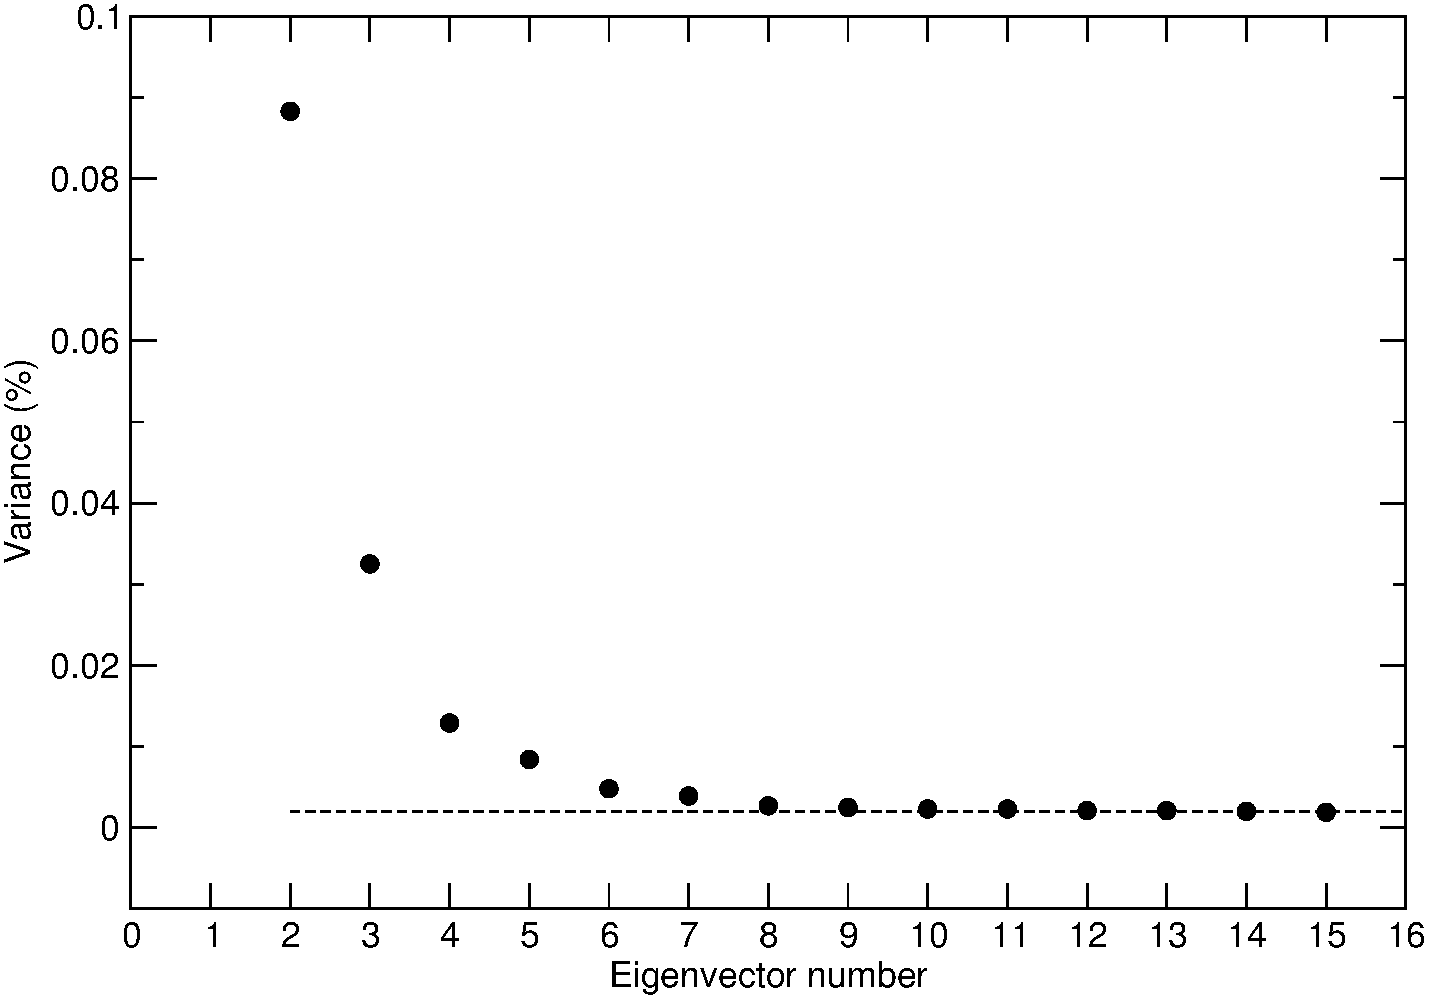
\includegraphics[width=0.7\textwidth]{figuras/figSteiner2009fig1.pdf}
    \caption[{\em Scree test} na galáxia NGC 4736.]
    {Scree test das primeiras 16 PCs do cubo de espectros da região central da galáxia NGC 4736. Retirado de
    S09.}
    \label{fig:S09scree}
\end{figure}

\begin{figure}
    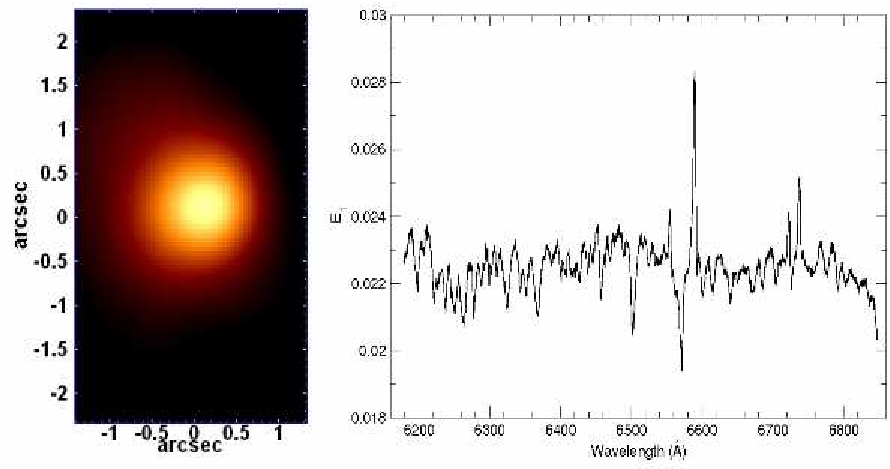
\includegraphics[width=0.9\textwidth]{figuras/figSteiner2009figA1.pdf}
    \caption[Tomograma e autoespectro 1 da galáxia NGC 4736.]
    {Autoespectro 1 e seu respectivo tomograma. Retirado de S09.}
    \label{fig:S09eigspec1}
\end{figure}

\begin{figure}
    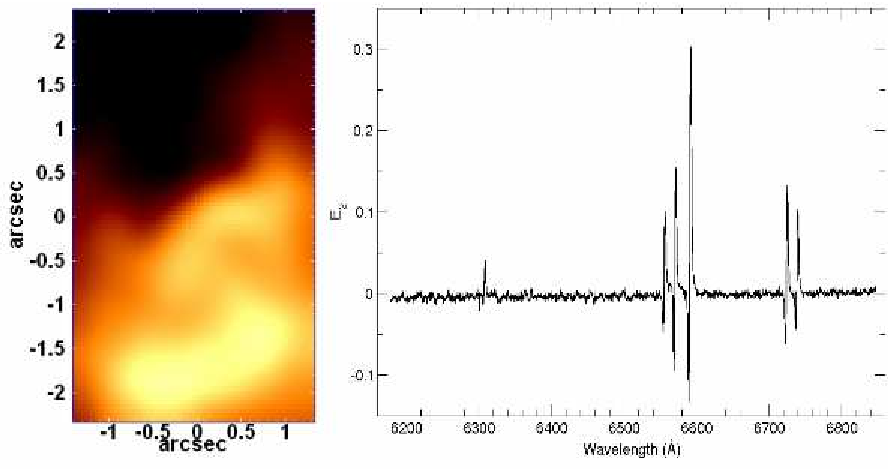
\includegraphics[width=0.9\textwidth]{figuras/figSteiner2009figA2.pdf}
    \caption[Tomograma e autoespectro 2 da galáxia NGC 4736.]
    {Autoespectro 2 e seu respectivo tomograma. Retirado de S09.}
    \label{fig:S09eigspec2}
\end{figure}

\begin{figure}
    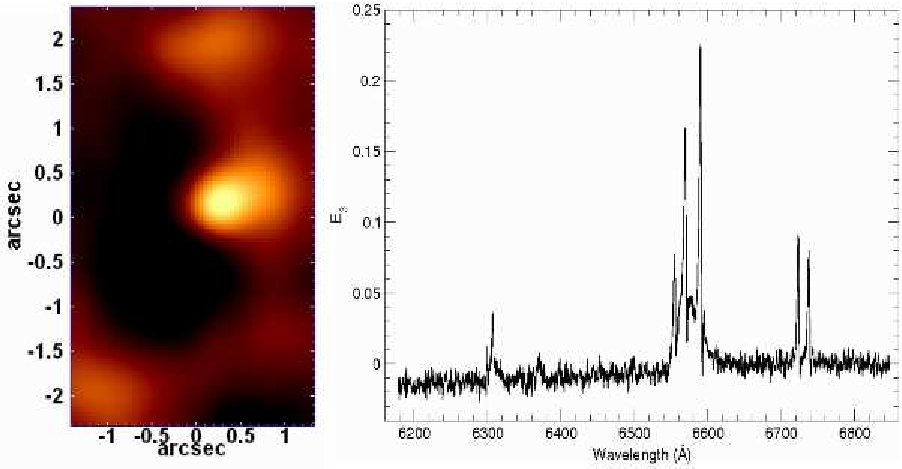
\includegraphics[width=0.9\textwidth]{figuras/figSteiner2009figA3.pdf}
    \caption[Tomograma e autoespectro 3 da galáxia NGC 4736.]
    {Autoespectro 3 e seu respectivo tomograma. Retirado de S09.}
    \label{fig:S09eigspec3}
\end{figure}

%\subsection{Reflexao da luz de um AGN escondido em NGC 7097}

%{\bf\ojo A FAZER!! Ricci et al 2011. Figs 3 e 5. vais precisar da minha ajuda para entender esse assunto de
%reflexao ... le o paper e depois falamos}

\section{Diferen\c{c}as com respeito ao trabalho anterior}

O exemplo acima nos motiva a aplicar esta mesma técnica aos cubos de dados do CALIFA, e o resto desta dissertação
apresenta nossos experimentos nesse sentido. Cumpre ressaltar, contudo, que o tipo de dados que analisaremos difere
bastante dos dados analisados até agora com essa nova ferramenta.

Essas diferenças são tanto de caráter observacional, como metodológico e físico. Para começo de conversa, S09 trabalham
com dados do Gemini (8m) com $3 \times 20$ min de integração, enquanto nossos dados vêm de integrações de tipicamente
30 min para o V1200 e 15 min para o V500 com $2\sim3$ exposições, no telescópio de 3.5m do observatório de Calar Alto.

Além disso, eles aplicam técnicas de deconvolução das imagens com o algorítmo de Richardson-Lucy. Dado o pequeno {\em
FoV} do IFU do Gemini, o ganho com tais técnicas é perceptível. Não aplicaremos isso no nosso caso porque nosso {\em
FoV} é muito maior, e não esperamos grandes ganhos em resolução espacial com a aplicação de tais técnicas de
deconvolução espacial.

Como dito na Seção \ref{sec:CALePyC:Apresent} a escala e resolução espacial de nossos dados difere brutalmente daquelas
nos trabalhos acima resumidos: $3^{\prime\prime} \times 5^{\prime\prime}$ e resolução de $0.47^{\prime\prime}$ no Gemini
contra $74^{\prime\prime} \times 64^{\prime\prime}$ e resolução de $\sim3.7^{\prime\prime}$ no CALIFA. Portanto, o {\em
FoV} estudado por S09 equivalem a aproximadamente $\sim2$ elementos de resolução do CALIFA! Isto de cara mostra que a
ciência que podemos obter com Tomografia PCA aplicada aos dados do CALIFA não será a mesma que aquela estudada por S09.

Em resumo, apesar de inspirado diretamente pelos resultados de S09, este estudo difere muito dos trabalhos deles. Estas
diferenças ficarão evidentes já a partir do próximo capítulo, onde apresentamos nossos primeiros resultados e discutimos
algumas variações com respeito ao processamento de S09, que decidimos fazer para melhor se adequar ao contexto de dados
do CALIFA.

%% End of this chapter